\begin{figure}[h]
    \centering
    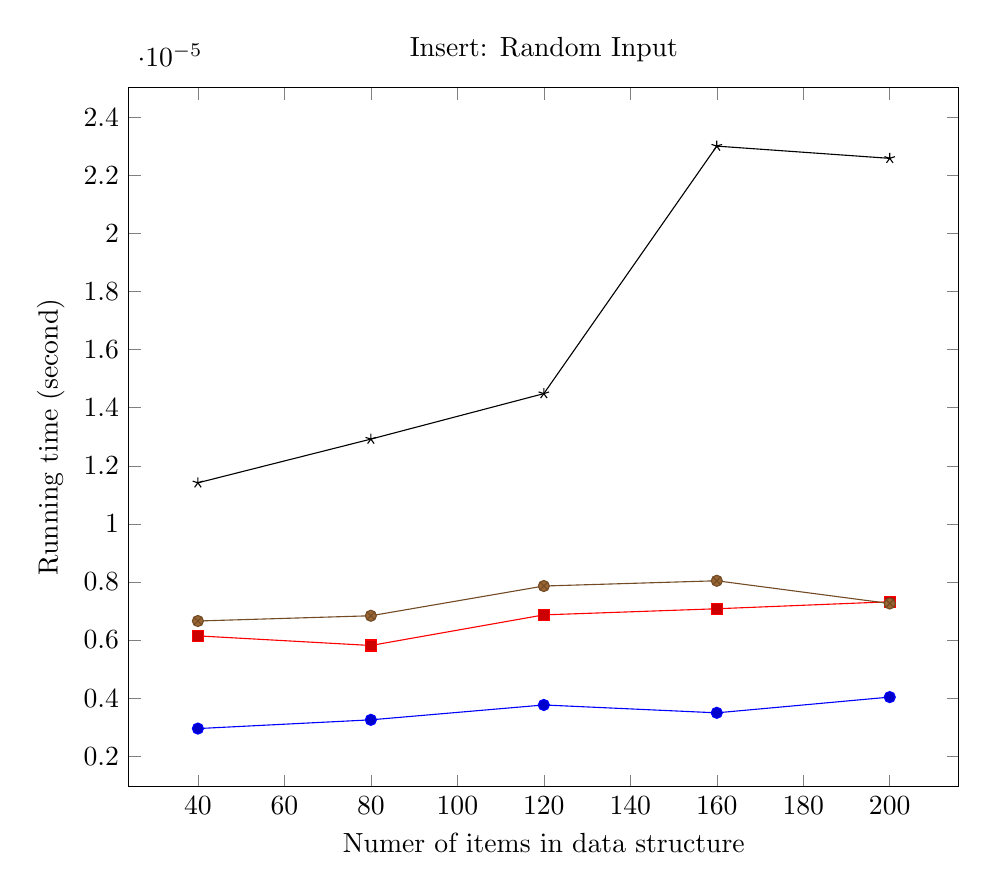
\begin{tikzpicture}
        \begin{axis}[
            xlabel={Numer of items in data structure},
            ylabel={Running time (second)},
            title={Insert: Random Input},
            width=\textwidth
        ]
		\addplot coordinates {
			(40, 2.9515183001664012e-06)
			(80, 3.2526936369180715e-06)
			(120, 3.764691709395927e-06)
			(160, 3.493633906319414e-06)
			(200, 4.0357495124724405e-06)
		};
		\addplot coordinates {
			(40, 6.143976869734139e-06)
			(80, 5.812683999307285e-06)
			(120, 6.866797677938189e-06)
			(160, 7.077620413664318e-06)
			(200, 7.318560683065682e-06)
		};
		\addplot coordinates {
			(40, 6.655974942211974e-06)
			(80, 6.836680144262954e-06)
			(120, 7.860676289218709e-06)
			(160, 8.041381491269601e-06)
			(200, 7.2583256157153844e-06)
		};
		\addplot coordinates {
			(40, 1.1414545262888354e-05)
			(80, 1.2920421946646839e-05)
			(120, 1.4486533697755447e-05)
			(160, 2.3009795727827775e-05)
			(200, 2.258815025637552e-05)
		};
        \legend{}
        \end{axis}
    \end{tikzpicture}
    \caption{Average of 0 operations, benchmarked every 0, starting at 0.}
\end{figure}